
\chapter{Parallel Transport Tool}\label{ch:parallel_transport}

In this section we present parallel transport for the finite dimensional Lie group and we make the assumption that obtained results hold in the infinite dimensional case.




% % % % % % % % % % % % % % % % % % % % % % % % % % % % % % % % % % % % % %
% % SUBSECTION
% % % % % % % % % % % % % % % % % % % % % % % % % % % % % % % % % % % % % % 
\section{Connections and Geodesics}

Given a Lie Group $\mathbb{G}$, a connection $\nabla$ is an operator which assign to each vector field $U$ in $\mathcal{V}(\mathbb{G})$ the map
\begin{align*}
\nabla_{U} : \mathcal{V}(\mathbb{G}) & \longrightarrow  \mathcal{V}(\mathbb{G}) &   \\
V &\longmapsto  \nabla_{U}V
\end{align*}
such that for all $f,g$ in $\mathcal{C}^{\infty}(\mathbb{G})$ and for all $V,W$ in $\mathcal{V}(\mathbb{G})$ the following conditions are satisfied:
\begin{enumerate}
	\item $ \nabla_{fU + gV} = f\nabla_{U} + g\nabla_{V}$
	\item $\nabla_{U}(fV) = f \nabla_{U}(V) + (Uf)V $
\end{enumerate}
where in the second condition we have used the structure of  $\mathcal{C}^{\infty}$-module of $\mathbb{G}$ and the fact that 
\begin{align*}
Uf: \mathbb{G} & \longrightarrow  \mathbb{R}    \\
p &\longmapsto  U_{p}f
\end{align*}
Geometrically the vector field $\nabla_{U}(V)$ associates at each point of the manifold the projection on the tangent plane of the covariant derivative of $U$ in the direction of $V$. The definition seems cryptic but the connection appears to be that general tool that provides geodesics and curvature over manifold on which no Riemannian metric has been defined \cite{do1992riemannian}.
In fact on a Lie group $\mathbb{G}$ a \emph{geodesic} between two of its points $p$ and $q$ can be defined as the curve $\gamma$ such that:
\begin{align*}
\gamma:[0,1] \longrightarrow \mathbb{G} \qquad \gamma(0)=p,~ \gamma(1) = p,~ \nabla_{\dot{\gamma}}\dot{\gamma} = 0 
\end{align*} 
Note that in this case the concept of geodesic did not involves any metric defined on the surface of the manifold. If also a Riemannian metric is defined on $\mathbb{G} $, then geodesics defined by the metric coincides with the geodesics defined by the connection only for the particular Levi-Civita connection.
A connection is said to be left invariant if it is closed for left invariant vector fields, i.e. if for any $V, W \in Left\mathcal{V}(\mathbb{G}) $ their connection $ \nabla_{U}V$ is still left invariant.

% % % % % % % % % % % % % % % % % % % % % % % % % % % % % % % % % % % % % %
% % SUBSECTION
% % % % % % % % % % % % % % % % % % % % % % % % % % % % % % % % % % % % % % 
\section{Affine Exponential, Logarithm and Log-Composition}
If $\mathbb{G} $ is endowed with a connection $\nabla$, then a new kind of exponential from the Lie algebra to the Lie group can be defined, using geodesics. This time the tangent plane that defines the Lie algebra is considered at the generic point $p$ of the Lie group and $\mathbf{v} \in T_{p}\mathbb{G}\simeq \mathfrak{g}$ is a tangent vector at the point $p$: 
\begin{align*}
	\exp :  \mathbb{G}  \times \mathfrak{g}     &\longrightarrow \mathbb{G}  
	\\ 
	(p,\mathbf{v}) &\longmapsto \exp_{p}(\mathbf{v})  = \gamma(1; p,\mathbf{v})
\end{align*}
The curve $\gamma(t;p,\mathbf{v}) = \gamma(t)$ on on $\mathbb{G}$ is the unique one with the following features:  
\begin{align*}
  \gamma(0) = p\qquad  \dot{\gamma}(0) =  \mathbf{v} \qquad \nabla_{\dot{\gamma}}\dot{\gamma} = 0 
\end{align*}
To distinguish the affine $\exp$ and $\log$ from the Lie $\exp$ and $\log$ presented in the previous chapter, the affine will always have the subscript of the point of application even when it is the identity.\\
The following properties hold:
\begin{enumerate}
	\item If $\nabla$ is a Cartan connection then $\exp_{e}$ and $\exp$ coincides.
	\item For all $p$ in $\mathbb{G}$, $\mathbf{v} \in T_{p}\mathbb{G}$ and $t$ real
	\begin{align*}
	 \exp _{p}(t\mathbf{v})  = \gamma(t; p,\mathbf{v})
	\end{align*}
	\item Given $\mathbf{u} \in T_{e}\mathbb{G}$, $\mathbf{v} \in T_{\exp _{e}(\mathbf{u})}\mathbb{G}$, exists a $\mathbf{w} \in T_{e}\mathbb{G}$ such that 
	\begin{align*}
	\exp_{e}(\mathbf{w})  = \exp_{\exp _{e}(\mathbf{u})}(\mathbf{v}) \circ  \exp _{e}(\mathbf{u})
	\end{align*}
	\item If $V$ is a unitary left-invariant vector field, then for $V_{e} \in T_{e}\mathbb{G}$
	\begin{align*}
	\exp_{e}(2V_{e})  = \exp_{\exp _{e}(V_{e})}(V_{\exp _{e}(V_{e})}) \circ  \exp _{e}(V_{e})
	\end{align*}
\end{enumerate}
Last two properties provides the intuitive idea that it is possible to move on the fiber bundle of the Lie group transporting in some sense a tangent vector defined at the identity on another tangent space. Certainly the Lie group possess a unique Lie algebra, as the tangent space at some point (the group's identity by convention), but two different tangent space (so two times the same Lie algebra structure) may not be oriented in the same way. \\
xxx parallel transport example on the sphere.\\
To approach the inverse of the affine exponential we consider the affine logarithm:
\begin{align*}
\log :  \mathbb{G}  \times \mathbb{G}   \longrightarrow T_{p}\mathbb{G}   \simeq \mathfrak{g} 
\\ 
(p,q) \longmapsto \log_{p}(q)  = \mathbf{v} 
\end{align*}
Where $\mathbf{v} $ is the vector at the tangent plane defined at $p$ such that the curve on $\mathbb{G} $ with the following features
\begin{align*}
\gamma(0) = p\qquad  \gamma(1) = q \qquad \nabla_{\dot{\gamma}}\dot{\gamma} = 0 
\end{align*}
has as its tangent in $p$ the vector $\mathbf{v}$.\\
xxx properties of affine log and exp xxx
Any Lie group $\mathbb{G}$ considered with a left-invariant connection $\nabla$ can be equipped with a metric,  based on the elements of its tangent space and on the log, and not necessarily coincident with the Riemannian one:
\begin{align*} 
\text{dist}(x,y) := \euclideanMetric{\log_{e}(x^{-1}\circ y) } \qquad \forall x, y \in \mathbb{G}
\end{align*}

\subsection{Definition of Affine Log-Composition}
We need to extend the definition of Lie log-composition to the Affine Log-composition. The first step is to extend the definition of internal cut locus of the Lie algebra, even when not centered at the zero. 
If the Lie algebra, considered as tangent space, is not considered at $e$ of $\mathbb{G}$ but at the point $p$ instead, we still have a diffeomorphism between a neighborhood of $\mathbf{0}$ in $\mathfrak{g}$ to a neighborhood of $p$ in $\mathbb{G}$. The internal cut locus of $\mathfrak{g}$ this time is based on $p$ and it is denoted with $C_{\mathfrak{g}}(p)$.

Given a point $p_1$ and a vector $\mathbf{v}_{1}$ on its tangent plane $T_{p_1}\mathbb{G}$ the \emph{affine Log-composition} is defined as the operator operation $\tilde{\star} $ over the $\mathbb{G}$ fiber bundle such that 
\begin{align*}
\cdot ~ \tilde{\star} ~ \mathbf{v}_{1}  : T_{\exp_{p_1}(\mathbf{v}_{1})}\mathbb{G}  & \longrightarrow T_{p_1}\mathbb{G}   
\\
\mathbf{v}_{2}&\longmapsto \mathbf{v}_{2}~\tilde{\star}~ \mathbf{v}_{1}
=
\log_{p_1}(\exp_{\exp_{p_1}(\mathbf{v}_{1})}(\mathbf{v}_{2})\circ\exp_{p_1}(\mathbf{v}_{1}))
\end{align*}
Note that not necessarily $\mathbf{v}_{1}~\tilde{\star}~ \mathbf{v}_{2}$ is a vector belonging to the internal cut locus based on the starting point $p_{1}$.

% % % % % % % % % % % % % % % % % % % % % % % % % % % % % % % % % % % % % %
% % SUBSECTION
% % % % % % % % % % % % % % % % % % % % % % % % % % % % % % % % % % % % % % 
\section{Parallel Transport through Examples}
Parallel transport will play a role in the computation of both Lie and Affine log-composition.
\begin{definition}
	Let $\mathbb{G}$ be a finite dimensional connected Lie group defined with a connection $\nabla$. Given $p,q \in \mathbb{G}$ and $\gamma : [0,1] \rightarrow \mathbb{G}$ such that $\gamma(0) = p$ and $\gamma(1) = q$, then the vector $V_{p} \in T_{p}\mathbb{G}$, belonging to some vector field $V$ is parallel transported along $\gamma$ up to $T_{q}\mathbb{G}$ if for all $t \in  [0,1]$ $\nabla_{\dot{\gamma}}V_{\gamma(t)} = 0$.\\
	The parallel transport is the function that maps $V_{p}$ from $T_{p}\mathbb{G}$ to $T_{q}\mathbb{G}$ along $\gamma$:
	\begin{align*}
		\Pi(\gamma)_{p}^{q} :  T_{p}\mathbb{G} & \longrightarrow T_{q}\mathbb{G}  \\
		V_{p}&\longmapsto \Pi(\gamma)_{p}^{q}(V_{p}) = V_{q}
	\end{align*}
\end{definition}

\noindent
xxx examples of parallel transport: manifold as surfaces and matrices! Calculemus!

\begin{prop}[Inversion]
	$\mathbb{G}$ Lie group, $\nabla$ connection, $p,q\in\mathbb{G}$. Given $\gamma$ such that $\gamma(0)= p$, $\gamma(1)=q$ and $\dot{\gamma}(0)=\mathbf{u}\in T_{p}\mathbb{G}$, we have:
	\begin{align}
& \Pi(\gamma)_{p}^{q}(-\mathbf{u}) = -\Pi(\gamma)_{p}^{q}(\mathbf{u}) )\\
& p = \exp_{q}(\mathbf{u}) \Longleftrightarrow \phantom{z} q = \exp_{p}(-\Pi(\gamma)_{q}^{p}(\mathbf{u}))
	\end{align}
\end{prop}

\noindent
xxx proof, see notebook!


 \begin{figure}[htbp]
 	\centering
 	\begin{minipage}[b]{3cm}
 		\hspace{-4cm}
 		\centering
	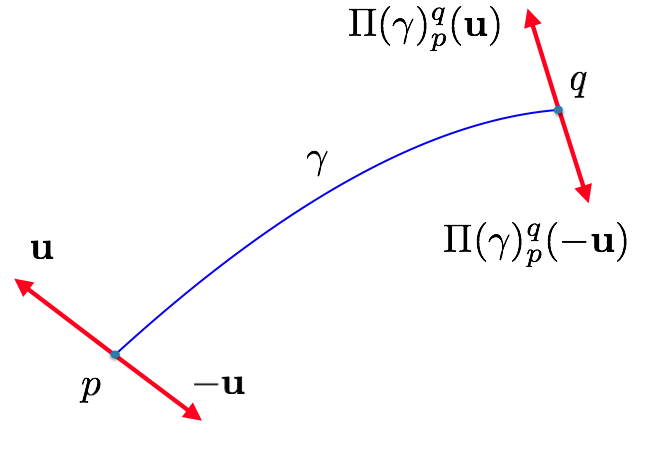
\includegraphics[width=6.5cm]{figures/inversion_1.png}
	\caption{First inversion property.}
	\label{fig:inversion_propr1}
 	\end{minipage}
 	\ \hspace{9mm} \
 	\begin{minipage}[b]{4cm}
 		\centering
	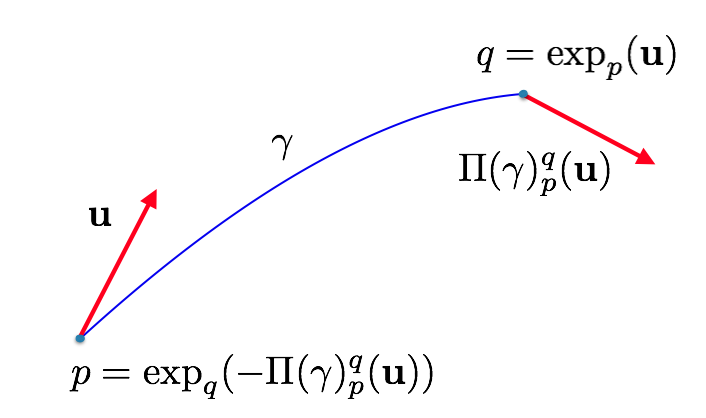
\includegraphics[width=6.5cm]{figures/inversion_2.png}
	\caption{Second inversion property.}
	\label{fig:inversion_propr2}
 	\end{minipage}
 \end{figure}


In the next property we explore how does behave the affine exponential expressed as a composition when changed of sign. It shows how the usefulness of the parallel transport in extending the property -if $\exp(\mathbf{w}) = \exp(\mathbf{u}) \circ \exp(\mathbf{v})$ then $\exp(\mathbf{-w}) = \exp(\mathbf{-v}) \circ \exp(\mathbf{-u})$- at the case of the affine exponentials.
\begin{prop}[change of signs of the composition for affine exponential]
	$\mathbb{G}$ Lie group, $\nabla$ connection, $a,b\in\mathbb{G}$, $\mathbf{u}\in T_{a}\mathbb{G}$, $\mathbf{v}\in T_{b}\mathbb{G}$. Let $\beta$ be the tangent curve to $\mathbf{u}$ at $a$ and $c= \exp_{b}(\mathbf{v})$. Given $\mathbf{w} \in T_{c}\mathbb{G}$ such that 
	\begin{align*}
		\exp_{a}(\mathbf{w}) = \exp_{b}(\mathbf{v}) \circ \exp_{a}(\mathbf{u})
	\end{align*}
	Then
	\begin{align*}
		\exp_{a}(-\mathbf{w}) = \exp_{\tilde{b}}(-\Pi(\beta)_{b}^{\tilde{b}}(\mathbf{v})) \circ \exp_{a}(-\mathbf{u})
	\end{align*}
	where $\tilde{b}$ is the affine exponential of $-\mathbf{u}$ or the element $\beta(-1)$.
\end{prop}


\begin{figure}[htbp]
	\centering
	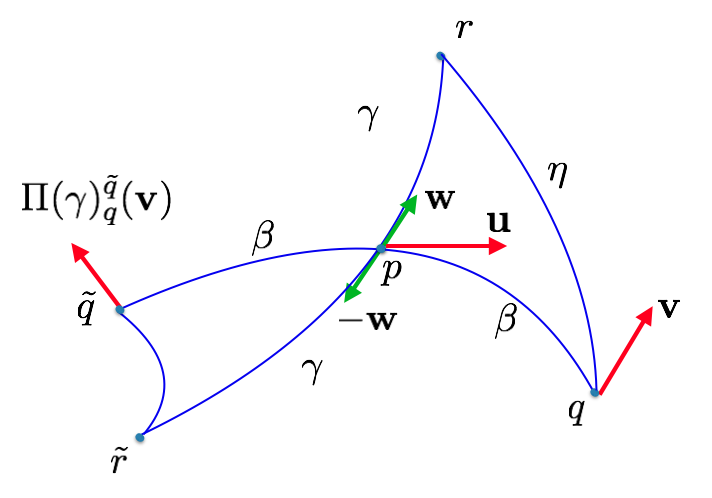
\includegraphics[width=9.5cm]{figures/sign_1.png}
	\caption{Change of sign property.}
	\label{fig:sign_propr}
\end{figure}


\noindent
xxx proof, see notebook!

\noindent
xxx Examples of these properties applied to real case!

% % % % % % % % % % % % % % % % % % % % % % % % % % % % % % % % % % % % % %
% % SUBSECTION
% % % % % % % % % % % % % % % % % % % % % % % % % % % % % % % % % % % % % % 
\section{Change of Base Formulas with and without Parallel Transport}
Using the derivative of the left-translation $L_{p}$ it is possible to bring back the $\exp$ and the $\log$ function based at the point $p$ of the manifold to the one evaluated at the identity using the following formulas:
\begin{align*}
	\log _{p}(q)  &= DL_{p}(e) \log _{e}(q)  \\
	\exp _{p}(\mathbf{u})  &= p\circ \exp_{e} (DL_{p}(e)^{-1} \mathbf{u})
\end{align*}
xxx Is this the same as the parallel transport? See examples and try to find a proof!!!


% % % % % % % % % % % % % % % % % % % % % % % % % % % % % % % % % % % % % %
% % SUBSECTION
% % % % % % % % % % % % % % % % % % % % % % % % % % % % % % % % % % % % % % 
\section{Parallel Transport in Practice: Schild's Ladder and Pole Ladder}




\begin{lemma}
	$\mathbb{G}$ Lie group, $\nabla$ connection, $a\in\mathbb{G}$, $\mathbf{u}\in T_{e}\mathbb{G}$. Let $\gamma$ be a curve defined on $\mathbb{G}$ such that $\gamma(0) = e$, $\gamma(1) = a$, $\dot{\gamma}(0) =\mathbf{u}$. Let $\beta$ be the curve over $\mathbf{G}$ defined as $\beta(t) = a\circ \gamma(t)$, then the two following conditions hold:
	\begin{enumerate}
		\item If $\nabla$ is a Cartan connection then $\beta$ is a geodesic.
		\item For $\mathbf{u}_{a} := D(L_{a})_{e}(\mathbf{u}) \in T_{a}\mathbb{G}$:
		\begin{align}
		\exp_{a}(t\mathbf{u}_{b}) = b\circ \exp_{e}( t D(L_{a^{-1}})_{a}(\mathbf{u}_{a}) ) = b\circ \exp_{e}(t\mathbf{u})
		\end{align}
	\end{enumerate}
\end{lemma}

\noindent
xxx proof, see notebook!

\begin{figure}[htbp]
	\centering
	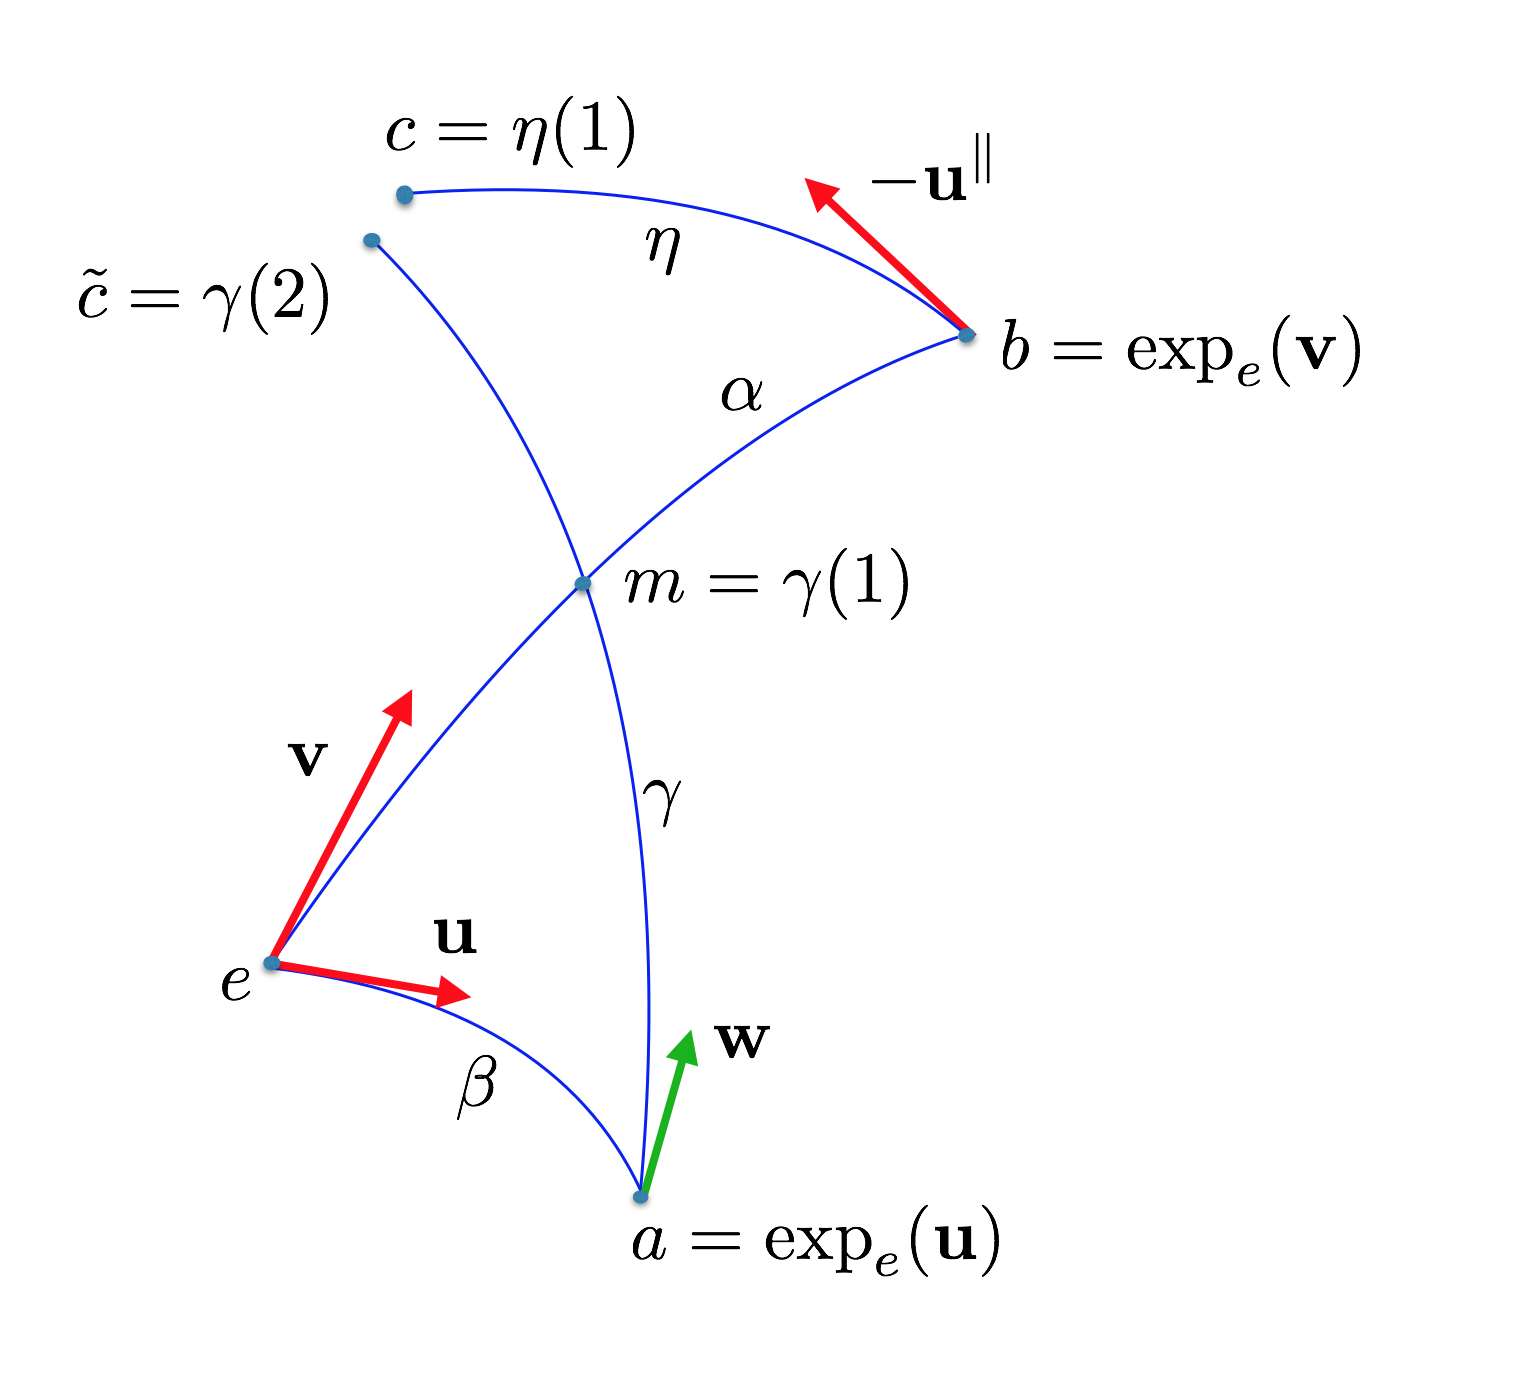
\includegraphics[width=9.5cm]{figures/theorem_pict.png}
	\caption{Pole ladder applied to parallel transport.}
	\label{fig:theorem_pict}
\end{figure}

\begin{theorem}\label{th:local_approximation_theorem}
	Let $\mathbb{G}$ be a finite dimensional connected Lie group defined with a Cartan connection $\nabla$. 
	If, for each couple of linearly independent vectors $\mathbf{u}, \mathbf{v} \in T_{e}\mathbb{G}$, we consider the following elements:
	\begin{align*}
	a= \exp_{e}(\mathbf{u}) 
	\quad & \quad  
	b= \exp_{e}(\mathbf{v}) \\
	\mathbf{u}^{\parallel} = & \Pi(\alpha)_{e}^{b}(\mathbf{u})\\
	\gamma : [0,1] \rightarrow \mathbb{G} &\quad \gamma(0) = e \quad \dot{\gamma}(0) = \mathbf{v}
	\end{align*}
	Then, for $\mathbf{u}_{e}^{\parallel} := D(L_{b^{-1}})_{e}( -\Pi(\alpha)_{a}^{b}(\mathbf{u}))$, the approximation
	\begin{align*}
	\exp_{e}(\mathbf{u}_{e}^{\parallel}) 
	\simeq
	\exp_{e}\big(\frac{\mathbf{v}}{2}\big)   
	\circ  \exp_{e}(\mathbf{u}) 
	\circ \exp_{e}\big(-\frac{\mathbf{v}}{2}\big)
	\end{align*}
	holds.
\end{theorem}

\begin{proof}
	As a consequence of the construction we have the following considerations:
	\begin{align*}
	\gamma(t) &= \exp(t\mathbf{w}) 
	= 
	a \circ \exp_{e}(D(L_{ba^{-1}})_{e}(t\mathbf{w})) 
	= 
	\exp_{e}(\mathbf{u})  \circ \exp_{e}(D(L_{a^{-1}})_{e}(t\mathbf{w})) 
	\\
	m &= \alpha(\frac{1}{2}) 
	= \exp_{e}\big(\frac{\mathbf{v}}{2}\big) = \gamma(1) = \exp_{a}(\mathbf{w})
	\\
	\exp_{e}&(D(L_{a^{-1}})_{e}(\mathbf{w})) = \exp_{e}(-\mathbf{u}) \circ  \exp_{e}\big(\frac{\mathbf{v}}{2}\big) 
	\end{align*}
	Let $\eta$ be the integral curve of  $-\Pi(\alpha)_{a}^{b}(\mathbf{u})$ starting at $b$. If $c := \eta(1)$ and $\tilde{c} := \gamma(1)$, then on one side we have:
	\begin{align*}
	\tilde{c} = \gamma(1) &= \exp_a(2\mathbf{w}) = a \circ\exp_{e}(D(L_{a^{-1}})_{e}(2\mathbf{w})) \\
	&= \exp_{e}(\mathbf{u})\circ\exp_{e}(D(L_{a^{-1}})_{e}(\mathbf{2w})) \\
	&= \exp_{e}(\mathbf{u})\circ\exp_{e}(2D(L_{a^{-1}})_{e}(\mathbf{w})) \\
	&= \exp_{e}(\mathbf{u})\circ \big(\exp_{e}(D(L_{a^{-1}})_{e}(\mathbf{w})) \big)^2\\
	&=  \exp_{e}(\mathbf{u})\circ \big(  \exp_{e}(-\mathbf{u}) \circ  \exp_{e}(\frac{\mathbf{v}}{2}) \big)^2\\
	&=   \exp_{e}\big(\frac{\mathbf{v}}{2}\big)   
	\circ  \exp_{e}(-\mathbf{u}) 
	\circ \exp_{e}\big(\frac{\mathbf{v}}{2}\big) 
	\end{align*}
	On the other side:
	\begin{align*}
	c = \eta(1) &= \exp_{b}(-\mathbf{u}^{\parallel}) = b \circ\exp_{e}(D(L_{b^{-1}})_{e}(-\mathbf{u}^{\parallel})) \\
	&= \exp_{e}(\mathbf{v}) \circ\exp_{e}(D(L_{b^{-1}})_{e}(-\mathbf{u}^{\parallel})) \\
	&= \exp_{e}(\mathbf{v}) \circ\exp_{e}(-\mathbf{u}_{e}^{\parallel}) 
	\end{align*}
	where $D(L_{b^{-1}})_{e}(\mathbf{u}^{\parallel})$ has been written $\mathbf{u}_{e}^{\parallel}$ for brevity.
	If we consider $c\simeq \tilde{c}$ it follows that:
	\begin{align*}
	\exp_{e}\big(\frac{\mathbf{v}}{2}\big)   
	\circ  \exp_{e}(-\mathbf{u}) 
	\circ \exp_{e}\big(\frac{\mathbf{v}}{2}\big)
	\simeq
	\exp_{e}(\mathbf{v}) \circ\exp_{e}(-\mathbf{u}_{e}^{\parallel}) 
	\end{align*}
	which implies
	\begin{align*}
	\exp_{e}(-\mathbf{u}_{e}^{\parallel}) 
	&\simeq
	\exp_{e}(-\mathbf{v}) 
	\circ \exp_{e}\big(\frac{\mathbf{v}}{2}\big)   
	\circ  \exp_{e}(-\mathbf{u}) 
	\circ \exp_{e}\big(\frac{\mathbf{v}}{2}\big)
	\\
	\exp_{e}(-\mathbf{u}_{e}^{\parallel}) 
	&\simeq
	\exp_{e}\big(-\frac{\mathbf{v}}{2}\big)   
	\circ  \exp_{e}(-\mathbf{u}) 
	\circ \exp_{e}\big(\frac{\mathbf{v}}{2}\big)
	\end{align*}
	As a consequence of property of the signs inversion it follows that
	\begin{align*}
	\exp_{e}(\mathbf{u}_{e}^{\parallel}) 
	\simeq
	\exp_{e}\big(\frac{\mathbf{v}}{2}\big)   
	\circ  \exp_{e}(\mathbf{u}) 
	\circ \exp_{e}\big(-\frac{\mathbf{v}}{2}\big)
	\end{align*}
\end{proof} 

\begin{corollary}
	xxx attempt to measure the error in the formula... to be done in a more effective way!
	If, with previous notations, the condition (1) is an approximation
	\begin{align*}
	\exp_{C}(\frac{\mathbf{k}}{2}) = \exp(\mathbf{\xi})\circ \exp_{M}(\frac{\mathbf{k}}{2}) 
	\end{align*}
	for some $ \mathbf{\xi}$ in  $\mathfrak{g}$ such that $\parallel\mathbf{\xi} \parallel < \delta$
	then the approximation has error
	\begin{align*}
	O(\parallel \delta\mathbf{u}^{\parallel} \parallel^{2} )  
	+ O(\parallel \mathbf{u} + \delta\mathbf{u}\parallel^{3})
	+ \text{xxx something that must be investigated depending on } \delta
	\end{align*}
\end{corollary}




